% PointMaze and AntMaze study that started 2026-11-11: a method that beats CleanRL PPO-RND.
% Every table body, both figures and every \BeatRnd... number are written by code/beat_rnd_tables.py from the run
% records (run it through code/beat_rnd_tables_job.py on a compute node); only the marked blocks are generated.
\clearpage
\section{PointMaze and AntMaze: beat CleanRL PPO-RND}
\label{sec:beat-rnd}

% Auto-generated by code/beat_rnd_tables.py
% >>> AUTO-GENERATED TABLE START: beat-rnd-numbers
\newcommand{\BeatRndFavouringMediumArrivalPlusOne}{$+0.0095$ $[+0.0015, +0.0178]$}
\newcommand{\BeatRndFavouringMediumStepCost}{$+0.0016$ $[-0.0031, +0.0062]$}
\newcommand{\BeatRndFavouringLargeArrivalPlusOne}{$+0.0153$ $[+0.0096, +0.0209]$}
\newcommand{\BeatRndFavouringLargeStepCost}{$+0.0112$ $[+0.0065, +0.0160]$}
\newcommand{\BeatRndNoBonusMediumStepCost}{$+0.004$ $[+0.002, +0.006]$}
\newcommand{\BeatRndConfirmationSeeds}{1{,}024}
\newcommand{\BeatRndAntCheckSteps}{16.8M}
\newcommand{\BeatRndAntCheckConfigurations}{48}
\newcommand{\BeatRndAntRunStepsSixteen}{67.1M}
\newcommand{\BeatRndAntBudgetRuleSixteen}{134M}
\newcommand{\BeatRndAntLatestRiseSixteen}{37M}
\newcommand{\BeatRndAntBestWSixteen}{0.0866}
\newcommand{\BeatRndAntBestLSixteen}{0.1027}
\newcommand{\BeatRndAntBestConfigurationSixteen}{intrinsic weight 0.0625, learning rate 0.0001, entropy 0.001}
\newcommand{\BeatRndAntRunStepsHundredTwentyEight}{134M}
\newcommand{\BeatRndAntBudgetRuleHundredTwentyEight}{268M}
\newcommand{\BeatRndAntLatestRiseHundredTwentyEight}{129M}
\newcommand{\BeatRndAntBestWHundredTwentyEight}{0.0770}
\newcommand{\BeatRndAntBestLHundredTwentyEight}{0.1293}
\newcommand{\BeatRndAntBestConfigurationHundredTwentyEight}{intrinsic weight 1, learning rate 0.01, entropy 0.001}
\newcommand{\BeatRndMediumStepCostStepSmallFirst}{$-0.3470$}
\newcommand{\BeatRndMediumStepCostStepZeroFirst}{$-0.3476$}
\newcommand{\BeatRndMediumStepCostStepSmallSecond}{$+0.0041$ $[-0.0017, +0.0103]$}
% <<< AUTO-GENERATED TABLE END: beat-rnd-numbers

\subsection{Task and protocol}
\label{sec:beat-rnd-protocol}

The goal is a method whose training curve of extrinsic return is ahead of a tuned CleanRL PPO-RND (the random
network distillation of Burda, Edwards, Storkey and Klimov, 2019) in all five mazes of \Cref{tab:beat-rnd-environments}, with statistical significance,
in one of two reward settings. The study has ten days from 2026-11-11: five for changes of the bonus, five for
changes of other parts of the learner. This section reports its state on 2026-11-13: PointMaze on two blocks of
validation seeds, AntMaze before any validation run.

\begin{table}[H]
\centering
\footnotesize
\setlength{\tabcolsep}{3pt}
\renewcommand{\arraystretch}{1.2}
\begin{tabular}{@{}>{\raggedright\arraybackslash}p{2.6cm}
?>{\raggedright\arraybackslash}p{1.95cm}
?>{\raggedright\arraybackslash}p{1.95cm}
?>{\raggedright\arraybackslash}p{1.95cm}
?>{\raggedright\arraybackslash}p{1.95cm}
?>{\raggedright\arraybackslash}p{1.95cm}@{}}
\blackrule
\textbf{Parameter} & \textbf{PointMaze Medium} & \textbf{PointMaze Large} & \textbf{AntMaze U-maze} &
\textbf{AntMaze Medium} & \textbf{AntMaze Large} \\
& \small this study & \small this study & \small this study & \small this study & \small this study \\
\blackrule
\multicolumn{6}{@{}l}{\textit{Map}} \\
\greyrule
open cells & $26$ & $46$ & $7$ & $26$ & $46$ \\
\greyrule
cell size & \multicolumn{2}{c?}{$1$\,m} & \multicolumn{3}{c}{$4$\,m} \\
\greyrule
start cell (row, column) & $(6, 1)$ & $(7, 1)$ & $(3, 1)$ & $(6, 1)$ & $(7, 1)$ \\
\greyrule
goal cell (row, column) & $(1, 6)$ & $(1, 10)$ & $(1, 1)$ & $(1, 6)$ & $(1, 10)$ \\
\greyrule
start and goal & \multicolumn{5}{>{\raggedright\arraybackslash}p{10.15cm}}{fixed, with no reset noise; the
goal is not observed} \\
\blackrule
\multicolumn{6}{@{}l}{\textit{Agent and episode}} \\
\greyrule
observation & \multicolumn{2}{>{\raggedright\arraybackslash}p{4.0cm}?}{$4$ numbers: position and velocity} &
\multicolumn{3}{>{\raggedright\arraybackslash}p{6.05cm}}{$29$ numbers of the ant's body} \\
\greyrule
physics & \multicolumn{2}{>{\raggedright\arraybackslash}p{4.0cm}?}{this platform's JAX point dynamics, checked
against Gymnasium-Robotics} & \multicolumn{3}{>{\raggedright\arraybackslash}p{6.05cm}}{MuJoCo's Warp
implementation inside MJX, $0.005$\,s time step, $10$ physics steps per environment step, a ceiling at the wall
tops that only the torso touches, an ant faster than $30$\,m/s or $100$\,rad/s is put back at the start} \\
\greyrule
step limit $H$ & \multicolumn{2}{c?}{$400$} & $700$ & \multicolumn{2}{c}{$1{,}000$} \\
\greyrule
goal event & \multicolumn{5}{>{\raggedright\arraybackslash}p{10.15cm}}{the agent within $0.45$\,m of the goal;
it ends the episode as a termination} \\
\blackrule
\end{tabular}
\caption{The five environments of the study. A value spanning several columns holds for each of them.}
\label{tab:beat-rnd-environments}
\end{table}

\paragraph{Rewards and episode ends.} Define $H$ as the step limit and $t$ as the step of an episode at which the
agent first comes within $0.45$\,m of the goal. Reaching the goal ends the episode as a termination: no value is
added after it. The step limit is a truncation: the extrinsic return continues with the value of the last state.
The intrinsic return runs on across both. The extrinsic discount is $0.999$ in both reward settings:
\begin{enumerate}
\item \textbf{Reward 1 on arrival:} reward $0$ per step and $1$ on arrival, so an episode returns $1$ when it
reaches the goal and $0$ otherwise.
\item \textbf{Step cost:} reward $-1/H$ per step and $0$ on arrival, so an episode returns $-(t-1)/H$ when it
reaches the goal and $-1$ otherwise.
\end{enumerate}

\paragraph{Learner.} Every run, the baseline's and every method's, is CleanRL's PPO with random network
distillation (RND): the clipped update with $4$ epochs of $4$ minibatches, clip $0.1$, rollouts of $128$ steps,
the learning rate annealed linearly to zero over the run's own budget, extrinsic and intrinsic discounts $0.999$
and $0.99$, extrinsic advantage weight $2$, the RND input whitened by running statistics and clipped to $\pm 5$
after $50$ rollouts of random actions, and the intrinsic reward divided by the running standard deviation of its
discounted sum. The one change from CleanRL, in every run: the predictor trains on the whole batch, not on a
quarter of it. PointMaze uses $4$ environments per policy, chosen by a check of $4$, $16$ and $128$ on PointMaze
Large. The intrinsic weight $\beta$ multiplies the intrinsic advantage.

\paragraph{Measures.} Define $K$ as the number of policies (seeds) of one configuration, $B$ as the budget in
environment steps per policy, $R_i(s)$ as the mean extrinsic return of the training episodes of policy $i$ that
end in the logging window containing step $s$ (a window with no finished episode takes the value of the window
before it), and $\Delta s$ as the number of steps of that window inside the range averaged. Define $T_i$ as the
training step of the first arrival of policy $i$, with $T_i = \infty$ when it never arrives. The primary measure
is the whole-curve mean $W$, with the final level $L$ beside it; the secondary measure is the mean capped
first-goal time $M$, with the share $F$ of policies that ever arrive as its tie-break:
\begin{align}
W(B) &= \frac{1}{K}\sum_{i=1}^{K}\frac{1}{B}\sum_{s\le B}R_i(s)\,\Delta s, &
L(B) &= \frac{1}{K}\sum_{i=1}^{K}\frac{1}{0.1B}\sum_{0.9B<s\le B}R_i(s)\,\Delta s,\\
M(B) &= \frac{1}{K}\sum_{i=1}^{K}\min(T_i,B), &
F(B) &= \frac{1}{K}\sum_{i=1}^{K}\mathbf{1}[T_i\le B].
\end{align}
$W$ is the area under the training curve divided by the budget, so it is higher when the goal is found sooner and
then kept: it measures discovery and optimization together. $M$ measures discovery alone, and smaller is better.
Each side, RND included, has its own configuration for each measure: the highest $W$ (ties: the higher $L$) and
the smallest $M$ (ties: the larger $F$). The two are never mixed in one row.

\paragraph{What ``beat'' means.} A method beats RND in one environment and reward setting when, on the same seeds,
both hold:
\begin{enumerate}
\item the 95\% interval of the paired difference in $W$ (method minus RND) lies entirely above zero;
\item the 95\% interval of the paired difference in $L$ does not lie entirely below zero.
\end{enumerate}
The method succeeds when it beats RND in all five environments with reward 1 on arrival, or in all five with the
step cost. A method whose 95\% interval of the difference in $M$ lies entirely below zero in all five environments
of one reward setting is noted as ahead on discovery; that is not part of success. Every interval is the $2.5\%$
and $97.5\%$ points of the means of $10{,}000$ resamples, with replacement, of the seeds both sides have. Two
runs with the same seed number on different cards part after their first rounding difference, so a seed number
pairs the start of two runs, not their paths.

\paragraph{Seeds, in the order they are used.}
\begin{enumerate}
\item \textbf{Development seeds $0$ to $15$:} every sweep. Each side's configurations for $W$ and for $M$ are
chosen here.
\item \textbf{First validation block, seeds $10000$ to $10255$:} a few leading configurations of each side. Each
side stands at its best configuration on this block, which is a second selection step on the same seeds.
\item \textbf{Second validation block, seeds $20000$ to $20255$:} nothing was chosen on these seeds. Each side
stands at the configuration fixed on the first block, RND at its own first-block best (``equal rules''). A
reading that is the best of several configurations counts only after this block.
\item \textbf{Fresh seeds from $30000$:} $1{,}024$ per configuration on PointMaze and $256$ on AntMaze. RND's
confirmation runs on them exist (\Cref{tab:beat-rnd-baseline}); no method has been run on them. They are kept for
the method as it stands at the end.
\end{enumerate}
On AntMaze a validation block has $128$ seeds (user decision of 2026-11-13).

\subsection{RND baseline on PointMaze}
\label{sec:beat-rnd-baseline}

RND's configurations were chosen on the development seeds in three sweeps: a first pass of $60$ configurations at
$50$M steps (intrinsic weight $4^{-6}$ to $4^{3}$ by factors of $4$, learning rate $10^{-4}$, $3\times10^{-4}$,
$10^{-3}$, entropy coefficient $0.001$ and $0.01$); a second pass around the best cell (weight by factors of
$2$, larger learning rates and entropy coefficients, intrinsic discount $0.99$ and $0.999$, clip $0.1$ and $0.2$);
and runs at the budget. The budget $B$ is twice the step at which the best three configurations reach $95\%$ of
their final level, rounded up to a power of two. A fourth sweep, toward larger weights and entropy coefficients,
chose RND's configuration for $M$. \Cref{tab:beat-rnd-baseline,tab:beat-rnd-baseline-step-cost} give both chosen
configurations and two reference rows on the fresh seeds.

\begin{table}[H]
\centering
\footnotesize
\setlength{\tabcolsep}{3pt}
\renewcommand{\arraystretch}{1.1}
% Auto-generated by code/beat_rnd_tables.py
% >>> AUTO-GENERATED TABLE START: beat-rnd-baseline-arrival
\begin{tabular}{@{}>{\raggedright\arraybackslash}p{5.4cm}>{\raggedright\arraybackslash}p{1.5cm}>{\raggedright\arraybackslash}p{1.5cm}>{\raggedright\arraybackslash}p{1.6cm}>{\raggedright\arraybackslash}p{1.3cm}@{}}
\toprule
row \newline configuration & $W$ $\uparrow$ & $L$ & $M$, thousand steps & policies that reach the goal \\
\midrule
\multicolumn{5}{@{}l}{\textbf{PointMaze Medium, reward 1 on arrival, budget 1.05M steps}} \\
RND, configuration for $W$ \newline \emph{intrinsic weight 2, learning rate 0.006, entropy 0.01} & {\bfseries\boldmath $0.932$} \newline $\pm 0.001$ & {\bfseries\boldmath $0.994$} \newline $\pm 0.001$ & \underline{$27$} \newline $\pm 0.78$ & 1,024 of 1,024 \\
RND, configuration for $M$ \newline \emph{intrinsic weight 4, learning rate 0.02, entropy 0.01} & \underline{$0.647$} \newline $\pm 0.004$ & \underline{$0.789$} \newline $\pm 0.004$ & {\bfseries\boldmath $17.4$} \newline $\pm 0.504$ & 1,024 of 1,024 \\
RND at CleanRL's defaults (reference) \newline \emph{intrinsic weight 1, learning rate 0.0001, entropy 0.001} & $0.585$ \newline $\pm 0.011$ & $0.788$ \newline $\pm 0.012$ & $210$ \newline $\pm 8.96$ & 957 of 1,024 \\
PPO without a bonus (reference) \newline \emph{intrinsic weight 0, learning rate 0.006, entropy 0.01} & $0.461$ \newline $\pm 0.013$ & $0.576$ \newline $\pm 0.015$ & $455$ \newline $\pm 14.5$ & 661 of 1,024 \\
\midrule
\multicolumn{5}{@{}l}{\textbf{PointMaze Large, reward 1 on arrival, budget 8.39M steps}} \\
RND, configuration for $W$ \newline \emph{intrinsic weight 2, learning rate 0.002, entropy 0.01} & {\bfseries\boldmath $0.881$} \newline $\pm 0.001$ & {\bfseries\boldmath $0.993$} \newline $\pm 0.000$ & \underline{$255$} \newline $\pm 4.99$ & 1,024 of 1,024 \\
RND at CleanRL's defaults (reference) \newline \emph{intrinsic weight 1, learning rate 0.0001, entropy 0.001} & \underline{$0.453$} \newline $\pm 0.010$ & \underline{$0.679$} \newline $\pm 0.014$ & $2{,}666$ \newline $\pm 86.2$ & 881 of 1,024 \\
RND, configuration for $M$ \newline \emph{intrinsic weight 64, learning rate 0.01, entropy 0.01} & $0.006$ \newline $\pm 0.000$ & $0.002$ \newline $\pm 0.000$ & {\bfseries\boldmath $136$} \newline $\pm 3.31$ & 1,024 of 1,024 \\
PPO without a bonus (reference) \newline \emph{intrinsic weight 0, learning rate 0.002, entropy 0.01} & $0.005$ \newline $\pm 0.002$ & $0.006$ \newline $\pm 0.002$ & $8{,}209$ \newline $\pm 35.8$ & 25 of 1,024 \\
\bottomrule
\end{tabular}
% <<< AUTO-GENERATED TABLE END: beat-rnd-baseline-arrival
\caption{RND with reward 1 on arrival on the fresh seeds from $30000$ (\BeatRndConfirmationSeeds{} per row), read
at the budget $B$ of each case. $W$ and $L$ (\Cref{sec:beat-rnd-protocol}) are means with their standard errors
under them; $M$ is in thousands of steps. Each row's configuration (``entropy'' is the entropy coefficient) was
chosen on the development seeds, except the two reference rows: RND at CleanRL's settings (learning rate
$10^{-4}$, entropy coefficient $0.001$, weight $1$) and PPO without a bonus at the learning rate and entropy
coefficient chosen for RND. Rows are sorted by $W$; per case and column the best value is bold and the second
underlined.}
\label{tab:beat-rnd-baseline}
\end{table}

\begin{table}[H]
\centering
\footnotesize
\setlength{\tabcolsep}{3pt}
\renewcommand{\arraystretch}{1.1}
% Auto-generated by code/beat_rnd_tables.py
% >>> AUTO-GENERATED TABLE START: beat-rnd-baseline-step-cost
\begin{tabular}{@{}>{\raggedright\arraybackslash}p{5.4cm}>{\raggedright\arraybackslash}p{1.5cm}>{\raggedright\arraybackslash}p{1.5cm}>{\raggedright\arraybackslash}p{1.6cm}>{\raggedright\arraybackslash}p{1.3cm}@{}}
\toprule
row \newline configuration & $W$ $\uparrow$ & $L$ & $M$, thousand steps & policies that reach the goal \\
\midrule
\multicolumn{5}{@{}l}{\textbf{PointMaze Medium, step cost, budget 1.05M steps}} \\
PPO without a bonus (reference) \newline \emph{intrinsic weight 0, learning rate 0.006, entropy 0.01} & {\bfseries\boldmath $-0.348$} \newline $\pm 0.001$ & {\bfseries\boldmath $-0.307$} \newline $\pm 0.000$ & \underline{$19.1$} \newline $\pm 0.469$ & 1,024 of 1,024 \\
RND, configuration for $W$ \newline \emph{intrinsic weight 0.00195312, learning rate 0.006, entropy 0.01} & \underline{$-0.352$} \newline $\pm 0.001$ & \underline{$-0.308$} \newline $\pm 0.000$ & $20.8$ \newline $\pm 0.619$ & 1,024 of 1,024 \\
RND, configuration for $M$ \newline \emph{intrinsic weight 4, learning rate 0.01, entropy 0.01} & $-0.370$ \newline $\pm 0.001$ & $-0.325$ \newline $\pm 0.001$ & {\bfseries\boldmath $14.1$} \newline $\pm 0.295$ & 1,024 of 1,024 \\
RND at CleanRL's defaults (reference) \newline \emph{intrinsic weight 1, learning rate 0.0001, entropy 0.001} & $-0.420$ \newline $\pm 0.004$ & $-0.345$ \newline $\pm 0.004$ & $30.3$ \newline $\pm 1.18$ & 1,023 of 1,024 \\
\midrule
\multicolumn{5}{@{}l}{\textbf{PointMaze Large, step cost, budget 33.6M steps}} \\
RND, configuration for $W$ \newline \emph{intrinsic weight 4, learning rate 0.002, entropy 0.01} & {\bfseries\boldmath $-0.732$} \newline $\pm 0.001$ & {\bfseries\boldmath $-0.716$} \newline $\pm 0.001$ & \underline{$208$} \newline $\pm 5.38$ & 1,024 of 1,024 \\
RND at CleanRL's defaults (reference) \newline \emph{intrinsic weight 1, learning rate 0.0001, entropy 0.001} & \underline{$-0.813$} \newline $\pm 0.003$ & \underline{$-0.786$} \newline $\pm 0.003$ & $2{,}723$ \newline $\pm 179$ & 1,001 of 1,024 \\
PPO without a bonus (reference) \newline \emph{intrinsic weight 0, learning rate 0.002, entropy 0.01} & $-0.847$ \newline $\pm 0.004$ & $-0.835$ \newline $\pm 0.004$ & $10{,}418$ \newline $\pm 467$ & 724 of 1,024 \\
RND, configuration for $M$ \newline \emph{intrinsic weight 8, learning rate 0.0045, entropy 0.01} & $-0.884$ \newline $\pm 0.001$ & $-0.888$ \newline $\pm 0.002$ & {\bfseries\boldmath $131$} \newline $\pm 3.29$ & 1,024 of 1,024 \\
\bottomrule
\end{tabular}
% <<< AUTO-GENERATED TABLE END: beat-rnd-baseline-step-cost
\caption{RND with the step cost on the fresh seeds, read as in \Cref{tab:beat-rnd-baseline}.}
\label{tab:beat-rnd-baseline-step-cost}
\end{table}

\begin{enumerate}
\item \textbf{The sweep matters.} At CleanRL's own settings RND is far behind its swept configuration in every
case, and on PointMaze Large with reward 1 on arrival PPO without a bonus almost never reaches the goal.
\item \textbf{Discovery and optimization need different settings.} RND's configuration for $M$ reaches the goal
soonest but its $W$ on PointMaze Large is close to that of a policy that never arrives: a large intrinsic weight
keeps the policy away from the goal after it has found it. This is why $M$ has its own configurations and tables.
\item \textbf{On PointMaze Medium with the step cost the bonus does not help.} PPO without a bonus is ahead of RND
on $W$ by \BeatRndNoBonusMediumStepCost{} on the fresh seeds, and RND's chosen weight there is close to no bonus,
so a change of the bonus alone has little room in this case.
\item \textbf{PointMaze Medium with reward 1 on arrival} keeps learning rate $0.006$, chosen when two runs of
learning rate $0.01$ with the same seed numbers on two card models gave different whole-curve means; the baseline
folder's generated report now names $0.01$ as the development choice.
\end{enumerate}

\subsection{The method}
\label{sec:beat-rnd-method}

The method is RND with two changes of the bonus. The user decided on 2026-11-13 that the first change, the divisor
held from each policy's first arrival, counts as part of the method, and that the baseline stays plain RND.

\paragraph{Notation.} Define $g$ as RND's fixed random target network, $\phi(x)$ as the predictor's last hidden
features of the whitened input $x$ with a constant $1$ appended (the input of the bias), and $V$ as the
predictor's output layer, so that the predictor's output is $V^{\top}\phi(x)$. The bonus of a state is
$b = \tfrac12\lVert e\rVert^2$ with the error $e = V^{\top}\phi(x) - g(x)$. Define $F_t = 0.99\,F_{t-1} + b_t$
as the discounted sum of the bonus, kept per environment across episodes, and $\sigma$ as the running standard
deviation of all $F_t$ since the first rollout. RND's learner sees the intrinsic reward $b_t/\sigma$.

\paragraph{First change: the divisor held from the first arrival.} Define $k_i$ as the rollout that contains the
first arrival of policy $i$ and $\sigma_i(k)$ as its divisor in rollout $k$. The divisor is updated as in RND
through rollout $k_i$ and then keeps its value:
\begin{equation}
\sigma_i(k) = \sigma_i\bigl(\min(k, k_i)\bigr).
\end{equation}
A policy that never arrives is scored exactly as by RND. In RND the divisor shrinks together with the bonus, so
the learner keeps seeing an intrinsic reward of about the same size for the whole run. With the divisor held,
the intrinsic reward after the first arrival is the prediction error times a constant and falls away as the
predictor learns, and the final level rises (the $L$ columns of
\Cref{tab:beat-rnd-whole-arrival,tab:beat-rnd-whole-step-cost}).

\paragraph{How close this is to published practice.} A background search of about $30$ queries and $60$ pages
(not a systematic review) found no paper that proposes or evaluates stopping the updates of RND's reward divisor
part-way through training, but two public sources come close. Clemens Schwarke, Victor Klemm, Matthijs van der
Boon, Marko Bjelonic and Marco Hutter, ``Curiosity-Driven Learning of Joint Locomotion and Manipulation Tasks''
(Conference on Robot Learning, 2023), report that RND's running reward normalisation keeps the intrinsic reward
from falling towards zero, and run RND without it at a fixed weight; after the hold, the method's intrinsic reward
is of that form. The RND module of the RSL-RL library builds its reward normaliser so that it stops updating after
$10^{8}$ samples. The hold here differs in when it happens: at each policy's own first arrival, not after a fixed
count of samples or a fixed share of the run. The divisor held after one sixteenth of the run, which is closer to
the public code, is shown as a reference row in every result table.

\paragraph{Second change: the fast last layer inside the rollout.} Define $\eta \in [0, 1]$ as the step of the
fast last layer, $N$ as the number of environments of one policy, $\Phi_t$ as the $N$ rows $\phi(x_{t,j})^{\top}$
of the states $x_{t,1},\dots,x_{t,N}$ reached at step $t$ of a rollout, and $E_t$ as the $N$ rows of their errors.
At the start of each rollout a temporary copy $\tilde V$ of the output layer is made, and the rollout's steps are
scored in time order: the states of step $t$ get the bonus $\tfrac12\lVert \tilde V^{\top}\phi(x_{t,j}) -
g(x_{t,j})\rVert^2$, and then $\tilde V$ takes the smallest change that multiplies each of their errors by
$1-\eta$:
\begin{equation}
\tilde V \leftarrow \tilde V - \eta\,\Phi_t^{+}E_t,
\end{equation}
where $\Phi_t^{+}$ is the pseudo-inverse of $\Phi_t$ (computed with a small ridge). A state reached again later
in the same rollout therefore pays less. The copy is dropped at the end of the rollout; the predictor itself
trains only in PPO's epochs, as in RND. The step is chosen per case, as the one with the highest whole-curve mean on
the first validation block among $\eta \in \lbrace 0, 0.01, 0.03, 0.1 \rbrace$ (a rule fixed before the second blocks
were read): $\eta = 0$ (off) on PointMaze Medium with reward 1 on arrival, $\eta = 0.01$ on Medium with the step cost,
and $\eta = 0.03$ on the two Large cases.

\begin{table}[H]
\centering
\footnotesize
\setlength{\tabcolsep}{3pt}
\renewcommand{\arraystretch}{1.2}
\begin{tabular}{@{}>{\raggedright\arraybackslash}p{2.8cm}
?>{\raggedright\arraybackslash}p{3.4cm}
?>{\raggedright\arraybackslash}p{3.4cm}
?>{\raggedright\arraybackslash}p{3.4cm}@{}}
\blackrule
\textbf{Setting} & \textbf{RND (baseline)} & \textbf{the method, Medium} & \textbf{the method, Large} \\
& \small CleanRL PPO-RND & \small two PointMaze cases & \small two PointMaze cases \\
\blackrule
\multicolumn{4}{@{}l}{\textit{Shared}} \\
\greyrule
environment specification & \multicolumn{3}{>{\raggedright\arraybackslash}p{10.6cm}}{unchanged ---
\Cref{tab:beat-rnd-environments}} \\
\greyrule
learner & CleanRL PPO-RND with the predictor trained on the whole batch (\Cref{sec:beat-rnd-protocol}) &
\multicolumn{2}{c}{same} \\
\blackrule
\multicolumn{4}{@{}l}{\textit{Bonus}} \\
\greyrule
divisor of the bonus & running standard deviation of its discounted sum, updated for the whole run &
\multicolumn{2}{>{\raggedright\arraybackslash}p{7.0cm}}{the same statistic, held from the rollout of each
policy's first arrival} \\
\greyrule
fast last layer & N/A & off ($\eta = 0$) & step $\eta = 0.03$ throughout the run \\
\blackrule
\multicolumn{4}{@{}l}{\textit{Chosen per case}} \\
\greyrule
\textbf{learning rate, intrinsic weight, entropy coefficient} & {\bfseries\boldmath its own sweeps on the
development seeds, then its best of the configurations run on the first validation block} &
\multicolumn{2}{>{\raggedright\arraybackslash}p{7.0cm}}{\bfseries\boldmath the same, with the step $\eta$ chosen
among $0$, $0.01$, $0.03$ and $0.1$} \\
\blackrule
\end{tabular}
\caption{RND and the method. ``same'' denotes a value shared with the column on its left; ``N/A'' a setting that
does not apply. Bold rows are chosen per case; the chosen values are in the result tables.}
\label{tab:beat-rnd-settings}
\end{table}

\paragraph{Why the fast last layer runs throughout, at a small step.}
\begin{enumerate}
\item \textbf{At step $0.1$ it finds the goal much sooner and keeps it badly.} At its own configurations for $M$ it
is ahead of RND on $M$ (\Cref{tab:beat-rnd-discovery-arrival,tab:beat-rnd-discovery-step-cost}) with $W$ close to
that of a policy that never arrives; with the first-arrival hold, each side at its best on the first block, it is
behind RND on $W$ on both Medium cases (\Cref{tab:beat-rnd-others}).
\item \textbf{Stopping it at each policy's first arrival failed} (batch 11): with the divisor of the fast scores
held or left running, $W$ was behind RND in every case run, by up to $0.45$ (\Cref{tab:beat-rnd-others}). The diagnosis (64 seeds, PointMaze
Medium, weight $4$, short runs): RND's divisor remembers the predictor's first, large errors (about $93$ in the
first $2{,}048$ steps and about $60$ to $65$ around the first arrival), while the fast last layer's scores are
about $14$ times smaller from the start and the divisor built on them stays near $4$. After the switch the
predictor's own scores are divided by that small divisor, the learner sees $10$ to $20$ times RND's intrinsic
reward, and the policies go on covering the maze instead of turning to the goal. A larger spread of the actions,
a predictor left in another state and the switch itself were ruled out.
\item \textbf{A second divisor kept on the predictor's own scores removes the failure} (batch 13), and is then
ahead of RND on the first block in two cases (\Cref{tab:beat-rnd-others}); it was not clearly better than the arm
finally chosen in any case and was not taken to the second block. It stays as the explanation of the slow
settling, not as part of the method.
\item \textbf{Smaller steps throughout, with the first-arrival hold} (batch 12), move both measures toward the hold
alone: a smaller step loses less return after the arrival and finds the goal later. On the first block the step
with the highest $W$ is $0.03$ on both Large cases and $0$ on Medium with reward 1 on arrival. On Medium with the
step cost step $0.01$ has a first-block $W$ of \BeatRndMediumStepCostStepSmallFirst{} against
\BeatRndMediumStepCostStepZeroFirst{} for the hold alone, a difference far inside the noise; by the rule step
$0.01$ is the method's step there. On the second block step $0.01$ gives \BeatRndMediumStepCostStepSmallSecond{}
against RND in that case.
\end{enumerate}

\subsection{Results on the second validation block}
\label{sec:beat-rnd-results}

\begin{table}[H]
\centering
\footnotesize
\setlength{\tabcolsep}{2.5pt}
\renewcommand{\arraystretch}{1.1}
% Auto-generated by code/beat_rnd_tables.py
% >>> AUTO-GENERATED TABLE START: beat-rnd-whole-arrival
\begin{tabular}{@{}>{\raggedright\arraybackslash}p{3.0cm}>{\raggedright\arraybackslash}p{1.25cm}>{\raggedright\arraybackslash}p{2.45cm}>{\raggedright\arraybackslash}p{2.45cm}>{\raggedright\arraybackslash}p{1.25cm}>{\raggedright\arraybackslash}p{2.45cm}@{}}
\toprule
arm \newline configuration fixed on the first block & $W$ $\uparrow$, second block & $W$ minus RND, first block, each at its best & $W$ minus RND, second block & $L$, second block & $L$ minus RND, second block \\
\midrule
\multicolumn{6}{@{}l}{\textbf{PointMaze Medium, reward 1 on arrival}} \\
\textbf{the method}: divisor held from the first arrival, fast last layer at step 0 (off) \newline \emph{intrinsic weight 4, learning rate 0.006, entropy 0.01} & {\bfseries\boldmath $0.9404$} \newline $\pm 0.0030$ & {\bfseries\boldmath $+0.0085$} \newline $[+0.0010, +0.0160]$ & {\bfseries\boldmath $+0.0095$} \newline $[+0.0015, +0.0178]$ & {\bfseries\boldmath $0.9999$} \newline $\pm 0.0000$ & {\bfseries\boldmath $+0.0092$} \newline $[+0.0043, +0.0177]$ \\
divisor held after one sixteenth of the run (reference) \newline \emph{intrinsic weight 4, learning rate 0.006, entropy 0.01} & \underline{$0.9398$} \newline $\pm 0.0025$ & \underline{$+0.0033$} \newline $[-0.0042, +0.0109]$ & \underline{$+0.0090$} \newline $[+0.0023, +0.0159]$ & \underline{$0.9995$} \newline $\pm 0.0002$ & \underline{$+0.0088$} \newline $[+0.0038, +0.0173]$ \\
\cmidrule(l{0pt}r{0pt}){1-6}
CleanRL PPO-RND (baseline) \newline \emph{intrinsic weight 2, learning rate 0.006, entropy 0.01} & $0.9308$ \newline $\pm 0.0030$ & baseline & baseline & $0.9907$ \newline $\pm 0.0039$ & baseline \\
\midrule
\multicolumn{6}{@{}l}{\textbf{PointMaze Large, reward 1 on arrival}} \\
\textbf{the method}: divisor held from the first arrival, fast last layer at step 0.03 \newline \emph{intrinsic weight 2, learning rate 0.002, entropy 0.01} & {\bfseries\boldmath $0.8995$} \newline $\pm 0.0022$ & {\bfseries\boldmath $+0.0195$} \newline $[+0.0138, +0.0254]$ & {\bfseries\boldmath $+0.0153$} \newline $[+0.0096, +0.0209]$ & $0.9968$ \newline $\pm 0.0004$ & $+0.0041$ \newline $[+0.0030, +0.0054]$ \\
divisor held from the first arrival alone (reference) \newline \emph{intrinsic weight 2, learning rate 0.002, entropy 0.01} & $0.8839$ \newline $\pm 0.0025$ & $+0.0094$ \newline $[+0.0031, +0.0156]$ & \underline{$-0.0003$} \newline $[-0.0066, +0.0059]$ & {\bfseries\boldmath $0.9976$} \newline $\pm 0.0003$ & {\bfseries\boldmath $+0.0049$} \newline $[+0.0038, +0.0060]$ \\
divisor held after one sixteenth of the run (reference) \newline \emph{intrinsic weight 2, learning rate 0.002, entropy 0.01} & $0.8819$ \newline $\pm 0.0030$ & \underline{$+0.0095$} \newline $[+0.0040, +0.0151]$ & $-0.0023$ \newline $[-0.0098, +0.0043]$ & \underline{$0.9969$} \newline $\pm 0.0005$ & \underline{$+0.0042$} \newline $[+0.0028, +0.0055]$ \\
\cmidrule(l{0pt}r{0pt}){1-6}
CleanRL PPO-RND (baseline) \newline \emph{intrinsic weight 2, learning rate 0.002, entropy 0.01} & \underline{$0.8842$} \newline $\pm 0.0019$ & baseline & baseline & $0.9927$ \newline $\pm 0.0005$ & baseline \\
\bottomrule
\end{tabular}
% <<< AUTO-GENERATED TABLE END: beat-rnd-whole-arrival
\caption{Reward 1 on arrival: $W$ and $L$ on the second validation block (seeds $20000$ to $20255$), each arm at
the configuration that was its best for $W$ on the first block and RND at its own first-block best. Differences
are the arm minus RND on the same seeds with their 95\% intervals under them. The column ``first block'' gives the
same difference on seeds $10000$ to $10255$ with each side at its best there. Arms are sorted by $W$, RND below the
rule; per case and column the best value is bold and the second underlined.}
\label{tab:beat-rnd-whole-arrival}
\end{table}

\begin{table}[H]
\centering
\footnotesize
\setlength{\tabcolsep}{2.5pt}
\renewcommand{\arraystretch}{1.1}
% Auto-generated by code/beat_rnd_tables.py
% >>> AUTO-GENERATED TABLE START: beat-rnd-whole-step-cost
\begin{tabular}{@{}>{\raggedright\arraybackslash}p{3.0cm}>{\raggedright\arraybackslash}p{1.25cm}>{\raggedright\arraybackslash}p{2.45cm}>{\raggedright\arraybackslash}p{2.45cm}>{\raggedright\arraybackslash}p{1.25cm}>{\raggedright\arraybackslash}p{2.45cm}@{}}
\toprule
arm \newline configuration fixed on the first block & $W$ $\uparrow$, second block & $W$ minus RND, first block, each at its best & $W$ minus RND, second block & $L$, second block & $L$ minus RND, second block \\
\midrule
\multicolumn{6}{@{}l}{\textbf{PointMaze Medium, step cost}} \\
divisor held from the first arrival alone (reference) \newline \emph{intrinsic weight 1, learning rate 0.006, entropy 0.01} & {\bfseries\boldmath $-0.3470$} \newline $\pm 0.0015$ & $+0.0029$ \newline $[-0.0014, +0.0071]$ & {\bfseries\boldmath $+0.0065$} \newline $[+0.0012, +0.0122]$ & $-0.3069$ \newline $\pm 0.0006$ & $+0.0013$ \newline $[-0.0011, +0.0041]$ \\
divisor held after one sixteenth of the run (reference) \newline \emph{intrinsic weight 2, learning rate 0.006, entropy 0.01} & \underline{$-0.3477$} \newline $\pm 0.0012$ & {\bfseries\boldmath $+0.0042$} \newline $[+0.0005, +0.0080]$ & \underline{$+0.0058$} \newline $[+0.0007, +0.0115]$ & {\bfseries\boldmath $-0.3062$} \newline $\pm 0.0004$ & {\bfseries\boldmath $+0.0020$} \newline $[-0.0002, +0.0047]$ \\
\textbf{the method}: divisor held from the first arrival, fast last layer at step 0.01 \newline \emph{intrinsic weight 2, learning rate 0.006, entropy 0.01} & $-0.3494$ \newline $\pm 0.0018$ & \underline{$+0.0035$} \newline $[-0.0008, +0.0077]$ & $+0.0041$ \newline $[-0.0017, +0.0103]$ & \underline{$-0.3068$} \newline $\pm 0.0005$ & \underline{$+0.0014$} \newline $[-0.0009, +0.0042]$ \\
\cmidrule(l{0pt}r{0pt}){1-6}
CleanRL PPO-RND (baseline) \newline \emph{intrinsic weight 0.00195312, learning rate 0.006, entropy 0.01} & $-0.3535$ \newline $\pm 0.0024$ & baseline & baseline & $-0.3082$ \newline $\pm 0.0012$ & baseline \\
\midrule
\multicolumn{6}{@{}l}{\textbf{PointMaze Large, step cost}} \\
\textbf{the method}: divisor held from the first arrival, fast last layer at step 0.03 \newline \emph{intrinsic weight 8, learning rate 0.002, entropy 0.01} & {\bfseries\boldmath $-0.7216$} \newline $\pm 0.0016$ & \underline{$+0.0087$} \newline $[+0.0039, +0.0134]$ & {\bfseries\boldmath $+0.0112$} \newline $[+0.0065, +0.0160]$ & \underline{$-0.7056$} \newline $\pm 0.0016$ & \underline{$+0.0119$} \newline $[+0.0070, +0.0169]$ \\
divisor held after one sixteenth of the run (reference) \newline \emph{intrinsic weight 8, learning rate 0.002, entropy 0.01} & \underline{$-0.7232$} \newline $\pm 0.0011$ & {\bfseries\boldmath $+0.0095$} \newline $[+0.0057, +0.0137]$ & \underline{$+0.0095$} \newline $[+0.0051, +0.0141]$ & {\bfseries\boldmath $-0.7045$} \newline $\pm 0.0011$ & {\bfseries\boldmath $+0.0130$} \newline $[+0.0084, +0.0179]$ \\
divisor held from the first arrival alone (reference) \newline \emph{intrinsic weight 8, learning rate 0.003, entropy 0.01} & $-0.7255$ \newline $\pm 0.0023$ & $+0.0074$ \newline $[+0.0017, +0.0128]$ & $+0.0072$ \newline $[+0.0013, +0.0131]$ & $-0.7101$ \newline $\pm 0.0023$ & $+0.0074$ \newline $[+0.0013, +0.0135]$ \\
\cmidrule(l{0pt}r{0pt}){1-6}
CleanRL PPO-RND (baseline) \newline \emph{intrinsic weight 4, learning rate 0.002, entropy 0.01} & $-0.7328$ \newline $\pm 0.0020$ & baseline & baseline & $-0.7175$ \newline $\pm 0.0021$ & baseline \\
\bottomrule
\end{tabular}
% <<< AUTO-GENERATED TABLE END: beat-rnd-whole-step-cost
\caption{Step cost: $W$ and $L$ on the second validation block, read as in \Cref{tab:beat-rnd-whole-arrival}.}
\label{tab:beat-rnd-whole-step-cost}
\end{table}

\begin{figure}[H]
\centering
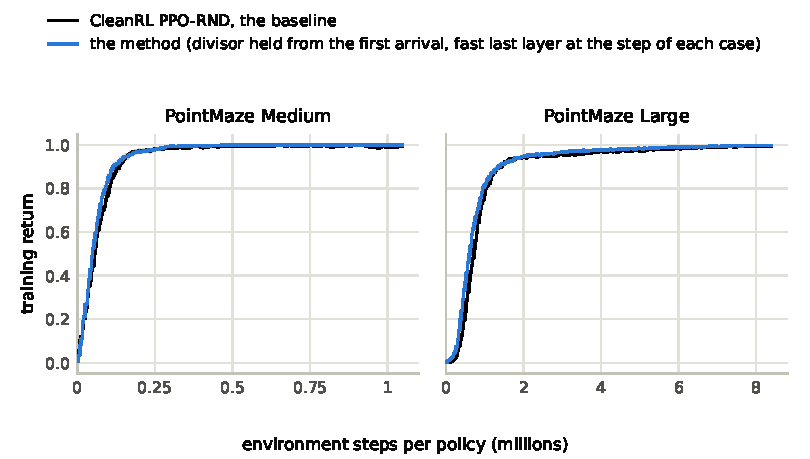
\includegraphics[width=\textwidth]{code/beat_rnd_plots/second-validation-block_training-return_arrival-plus-one.pdf}
\caption{Reward 1 on arrival: mean training return of the $256$ policies of the second validation block against
environment steps per policy, with a band of one standard error, for RND (black) and the method, each at the
configuration of \Cref{tab:beat-rnd-whole-arrival}. Drawn by \texttt{code/beat\_rnd\_tables.py}.}
\label{fig:beat-rnd-curves-arrival}
\end{figure}

\begin{figure}[H]
\centering
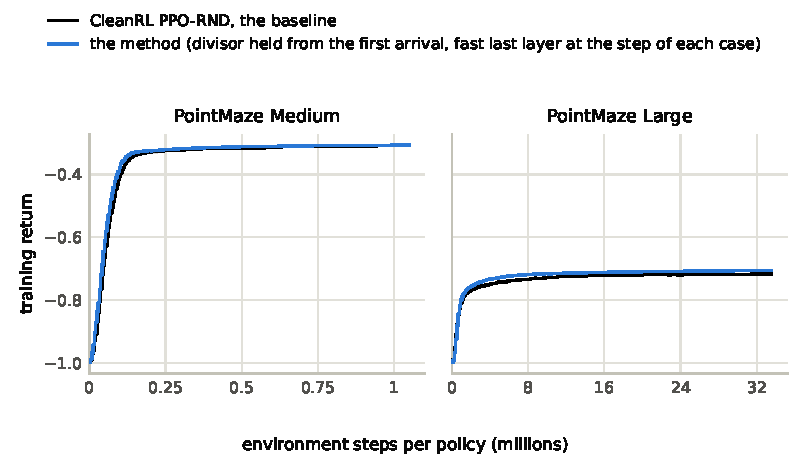
\includegraphics[width=\textwidth]{code/beat_rnd_plots/second-validation-block_training-return_step-cost.pdf}
\caption{Step cost: the curves of \Cref{fig:beat-rnd-curves-arrival} at the configurations of
\Cref{tab:beat-rnd-whole-step-cost}.}
\label{fig:beat-rnd-curves-step-cost}
\end{figure}

\begin{table}[H]
\centering
\footnotesize
\setlength{\tabcolsep}{2.5pt}
\renewcommand{\arraystretch}{1.1}
% Auto-generated by code/beat_rnd_tables.py
% >>> AUTO-GENERATED TABLE START: beat-rnd-discovery-arrival
\begin{tabular}{@{}>{\raggedright\arraybackslash}p{3.6cm}>{\raggedright\arraybackslash}p{1.45cm}>{\raggedright\arraybackslash}p{2.2cm}>{\raggedright\arraybackslash}p{2.2cm}>{\raggedright\arraybackslash}p{1.45cm}>{\raggedright\arraybackslash}p{1.3cm}@{}}
\toprule
arm \newline configuration with its smallest $M$ on the first block & $M$ $\downarrow$, second block & $M$ minus RND, first block, each at its best & $M$ minus RND, second block & $W$ at this configuration, second block & policies that reach the goal \\
\midrule
\multicolumn{6}{@{}l}{\textbf{PointMaze Medium, reward 1 on arrival}} \\
fast last layer at step 0.1, RND's running divisor (discovery arm) \newline \emph{intrinsic weight 16, learning rate 0.01, entropy 0.03} & {\bfseries\boldmath $13$} \newline $\pm 0.627$ & {\bfseries\boldmath $-4.99$} \newline $[-8.32, -2.37]$ & {\bfseries\boldmath $-3.78$} \newline $[-7.19, -0.924]$ & $0.1154$ & 256 of 256 \\
divisor held after one sixteenth of the run (reference) \newline \emph{intrinsic weight 4, learning rate 0.006, entropy 0.01} & $19.7$ \newline $\pm 1.13$ & $+3.47$ \newline $[-0.336, +6.84]$ & \underline{$+2.89$} \newline $[-0.835, +6.21]$ & $0.9398$ & 256 of 256 \\
\textbf{the method}: divisor held from the first arrival, fast last layer at step 0 (off) \newline \emph{intrinsic weight 4, learning rate 0.006, entropy 0.01} & $20.6$ \newline $\pm 1.12$ & \underline{$+0.993$} \newline $[-2.74, +4.35]$ & $+3.83$ \newline $[+0.451, +7.02]$ & $0.9404$ & 256 of 256 \\
\cmidrule(l{0pt}r{0pt}){1-6}
CleanRL PPO-RND (baseline) \newline \emph{intrinsic weight 4, learning rate 0.02, entropy 0.1} & \underline{$16.8$} \newline $\pm 1.43$ & baseline & baseline & $0.0075$ & 256 of 256 \\
\midrule
\multicolumn{6}{@{}l}{\textbf{PointMaze Large, reward 1 on arrival}} \\
fast last layer at step 0.1, RND's running divisor (discovery arm) \newline \emph{intrinsic weight 16, learning rate 0.006, entropy 0.03} & {\bfseries\boldmath $57.3$} \newline $\pm 2.47$ & {\bfseries\boldmath $-63.4$} \newline $[-75.2, -52]$ & {\bfseries\boldmath $-72.5$} \newline $[-84.6, -60.8]$ & $0.0010$ & 256 of 256 \\
\textbf{the method}: divisor held from the first arrival, fast last layer at step 0.03 \newline \emph{intrinsic weight 2, learning rate 0.002, entropy 0.01} & \underline{$118$} \newline $\pm 6.21$ & \underline{$+8.91$} \newline $[-8.23, +25.5]$ & \underline{$-12.1$} \newline $[-27.7, +4.01]$ & $0.8995$ & 256 of 256 \\
divisor held after one sixteenth of the run (reference) \newline \emph{intrinsic weight 2, learning rate 0.002, entropy 0.01}$^{\dagger}$ & $259$ \newline $\pm 10$ & $+93.9$ \newline $[+74.5, +113]$ & $+129$ \newline $[+108, +151]$ & $0.8819$ & 256 of 256 \\
divisor held from the first arrival alone (reference) \newline \emph{intrinsic weight 2, learning rate 0.002, entropy 0.01}$^{\dagger}$ & $266$ \newline $\pm 11.6$ & $+81.6$ \newline $[+61.3, +102]$ & $+136$ \newline $[+112, +161]$ & $0.8839$ & 256 of 256 \\
\cmidrule(l{0pt}r{0pt}){1-6}
CleanRL PPO-RND (baseline) \newline \emph{intrinsic weight 64, learning rate 0.006, entropy 0.01} & $130$ \newline $\pm 5.17$ & baseline & baseline & $0.0057$ & 256 of 256 \\
\bottomrule
\end{tabular}
% <<< AUTO-GENERATED TABLE END: beat-rnd-discovery-arrival
\caption{Reward 1 on arrival: $M$ in thousands of steps on the second validation block, each arm at the
configuration that was its best for $M$ on the first block, and RND at its own configuration for $M$ (from its
discovery sweep). A dagger marks an arm whose first-block best for $M$ was not run on the second block; it stands
at its best there, which favours it. The method and its two references were run only at configurations picked for
$W$, so their rows are not tuned for $M$; the discovery arm (the fast last layer at step $0.1$ with RND's running
divisor) was. Arms are sorted by $M$, RND below the rule; per case and column the best value is bold and the
second underlined (for $M$ and its differences the smallest).}
\label{tab:beat-rnd-discovery-arrival}
\end{table}

\begin{table}[H]
\centering
\footnotesize
\setlength{\tabcolsep}{2.5pt}
\renewcommand{\arraystretch}{1.1}
% Auto-generated by code/beat_rnd_tables.py
% >>> AUTO-GENERATED TABLE START: beat-rnd-discovery-step-cost
\begin{tabular}{@{}>{\raggedright\arraybackslash}p{3.6cm}>{\raggedright\arraybackslash}p{1.45cm}>{\raggedright\arraybackslash}p{2.2cm}>{\raggedright\arraybackslash}p{2.2cm}>{\raggedright\arraybackslash}p{1.45cm}>{\raggedright\arraybackslash}p{1.3cm}@{}}
\toprule
arm \newline configuration with its smallest $M$ on the first block & $M$ $\downarrow$, second block & $M$ minus RND, first block, each at its best & $M$ minus RND, second block & $W$ at this configuration, second block & policies that reach the goal \\
\midrule
\multicolumn{6}{@{}l}{\textbf{PointMaze Medium, step cost}} \\
fast last layer at step 0.1, RND's running divisor (discovery arm) \newline \emph{intrinsic weight 16, learning rate 0.01, entropy 0.03} & {\bfseries\boldmath $11.4$} \newline $\pm 0.459$ & {\bfseries\boldmath $-1.04$} \newline $[-2.35, +0.241]$ & {\bfseries\boldmath $-1.77$} \newline $[-3.12, -0.402]$ & $-0.9403$ & 256 of 256 \\
\textbf{the method}: divisor held from the first arrival, fast last layer at step 0.01 \newline \emph{intrinsic weight 2, learning rate 0.006, entropy 0.01} & $13.5$ \newline $\pm 0.628$ & $+1.4$ \newline $[+0.0507, +2.77]$ & \underline{$+0.291$} \newline $[-1.07, +1.69]$ & $-0.3494$ & 256 of 256 \\
divisor held from the first arrival alone (reference) \newline \emph{intrinsic weight 2, learning rate 0.006, entropy 0.01}$^{\dagger}$ & $14.7$ \newline $\pm 0.632$ & \underline{$+0.958$} \newline $[-0.349, +2.26]$ & $+1.46$ \newline $[+0.109, +2.91]$ & $-0.3472$ & 256 of 256 \\
divisor held after one sixteenth of the run (reference) \newline \emph{intrinsic weight 2, learning rate 0.006, entropy 0.01} & $15$ \newline $\pm 0.68$ & $+1.46$ \newline $[+0.281, +2.64]$ & $+1.82$ \newline $[+0.471, +3.18]$ & $-0.3477$ & 256 of 256 \\
\cmidrule(l{0pt}r{0pt}){1-6}
CleanRL PPO-RND (baseline) \newline \emph{intrinsic weight 4, learning rate 0.01, entropy 0.03} & \underline{$13.2$} \newline $\pm 0.497$ & baseline & baseline & $-0.5581$ & 256 of 256 \\
\midrule
\multicolumn{6}{@{}l}{\textbf{PointMaze Large, step cost}} \\
fast last layer at step 0.1, RND's running divisor (discovery arm) \newline \emph{intrinsic weight 16, learning rate 0.006, entropy 0.03} & {\bfseries\boldmath $58.2$} \newline $\pm 2.29$ & {\bfseries\boldmath $-61.3$} \newline $[-73.5, -49.6]$ & {\bfseries\boldmath $-62.7$} \newline $[-74.5, -51]$ & $-1.0000$ & 256 of 256 \\
\textbf{the method}: divisor held from the first arrival, fast last layer at step 0.03 \newline \emph{intrinsic weight 8, learning rate 0.002, entropy 0.01} & \underline{$89.3$} \newline $\pm 4.71$ & \underline{$-36.9$} \newline $[-50.9, -23.1]$ & \underline{$-31.6$} \newline $[-45.9, -17.4]$ & $-0.7216$ & 256 of 256 \\
divisor held from the first arrival alone (reference) \newline \emph{intrinsic weight 8, learning rate 0.003, entropy 0.01} & $152$ \newline $\pm 7.71$ & $+42.9$ \newline $[+24.2, +62.7]$ & $+31.5$ \newline $[+11.9, +52.1]$ & $-0.7255$ & 256 of 256 \\
divisor held after one sixteenth of the run (reference) \newline \emph{intrinsic weight 8, learning rate 0.002, entropy 0.01}$^{\dagger}$ & $184$ \newline $\pm 9.22$ & $+27.2$ \newline $[+9.57, +44.7]$ & $+63.3$ \newline $[+43.9, +83.7]$ & $-0.7232$ & 256 of 256 \\
\cmidrule(l{0pt}r{0pt}){1-6}
CleanRL PPO-RND (baseline) \newline \emph{intrinsic weight 8, learning rate 0.006, entropy 0.01} & $121$ \newline $\pm 5.71$ & baseline & baseline & $-0.9636$ & 256 of 256 \\
\bottomrule
\end{tabular}
% <<< AUTO-GENERATED TABLE END: beat-rnd-discovery-step-cost
\caption{Step cost: $M$ on the second validation block, read as in \Cref{tab:beat-rnd-discovery-arrival}.}
\label{tab:beat-rnd-discovery-step-cost}
\end{table}

\begin{enumerate}
\item \textbf{On the second block the method beats RND by the study's rule in three of the four PointMaze cases,
and is level in the fourth} (Medium with the step cost)
(\Cref{tab:beat-rnd-whole-arrival,tab:beat-rnd-whole-step-cost}): in three cases the interval of the difference
in $W$ lies above zero and the interval of the difference in $L$ does not lie below zero; on Medium with the step
cost the step the rule chooses ($0.01$) gives \BeatRndMediumStepCostStepSmallSecond, which includes zero. This is a
validation reading, not the verdict: the fresh seeds and all three AntMaze maps are still to come.
\item \textbf{The margin is small} (about $0.01$ of $W$). On PointMaze Medium with the step cost the divisor held
from the first arrival alone (step $0$, the reference row of \Cref{tab:beat-rnd-whole-step-cost}), whose
first-block mean was $0.0006$ below that of step $0.01$, is ahead of RND on the second block; choosing it there after
both second-block readings were known would be a choice made on the test seeds, so it is not counted. Against RND
at its best configuration on the second block itself, chosen after the block was read, the method's difference
there is \BeatRndFavouringMediumStepCost. In the other three cases
RND's first-block best is also its best on the second block.
\item \textbf{Where the gain comes from.} On PointMaze Medium with reward 1 on arrival mostly from the final
level: the held divisor brings $L$ to about $1$, where RND's stays below it. On the Large cases the fast last layer
adds an
earlier first arrival: the method's $M$ is near RND's own configuration for $M$ (level with reward 1 on arrival,
ahead with the step cost), while its $W$ stays at the top.
\item \textbf{Why a reading counts only after the second block.} The divisor held from the first arrival alone is
ahead of RND on PointMaze Large with reward 1 on arrival on the first block and level on the second
(\Cref{tab:beat-rnd-whole-arrival}); the fixed hold after one sixteenth of the run does the same.
\item \textbf{Discovery alone.} The fast last layer at step $0.1$, at its own configurations for $M$, is ahead of
RND at RND's configurations for $M$ on the second block in all four PointMaze cases, and on the first block in
three (level on Medium with the step cost). At those configurations its $W$ is near that of a policy that never
arrives. On PointMaze Medium the method itself reaches the goal later than RND's configuration for $M$.
\end{enumerate}

\subsection{What did not work}
\label{sec:beat-rnd-failed}

Each item is one idea, with one line of evidence. Items $1$ to $5$ are screens on the $16$ development seeds of
PointMaze Large with reward 1 on arrival (the batch summaries of batches 1 and 2; differences from RND in $W$);
the others are on the first validation block (\Cref{tab:beat-rnd-others}).
\begin{enumerate}
\item \textbf{Error length as the bonus} (the length of $e$ instead of $\tfrac12\lVert e\rVert^2$): $-0.040$ on
the development seeds, and behind RND at every weight on the first block, also with a held divisor.
\item \textbf{A fixed scale, an even start, and an even start with no divisor:} $-0.338$, $-0.698$ and $-0.557$.
\item \textbf{A scheduled last layer on the random body's features} (decay $0.5$, $0.75$, $1$): $-0.637$,
$-0.779$ and $-0.884$; fitting the visited inputs lowered the error everywhere.
\item \textbf{Local features (random Fourier) as the input of RND, and a scheduled last layer on them:} $-0.53$
to $-0.70$ and $-0.67$ to $-0.87$; every policy finds the goal, and none settles on it.
\item \textbf{Input statistics kept from the random-action rollouts:} $-0.054$; a wider input clip and a separate
predictor step size changed nothing measurable (within $\pm 0.006$).
\item \textbf{A slower predictor or a predictor at half speed, with the divisor held after one sixteenth:} ahead
in some cases and level in others, never better than the hold alone.
\item \textbf{All three parts together} (fast last layer, slower predictor, held divisor): behind RND on PointMaze
Medium with reward 1 on arrival.
\item \textbf{The fast last layer stopped at the first arrival without a second divisor:} far behind RND in every
case run (the cause is in \Cref{sec:beat-rnd-method}).
\item \textbf{The fast last layer at step $0.1$ throughout with the first-arrival hold:} behind RND on both Medium
cases; a smaller step replaced it.
\end{enumerate}

\begin{table}[H]
\centering
\footnotesize
\setlength{\tabcolsep}{2.5pt}
\renewcommand{\arraystretch}{1.1}
% Auto-generated by code/beat_rnd_tables.py
% >>> AUTO-GENERATED TABLE START: beat-rnd-others
\begin{tabular}{@{}>{\raggedright\arraybackslash}p{3.4cm}>{\raggedright\arraybackslash}p{2.45cm}>{\raggedright\arraybackslash}p{2.45cm}>{\raggedright\arraybackslash}p{2.45cm}>{\raggedright\arraybackslash}p{2.45cm}@{}}
\toprule
arm & \shortstack[l]{PointMaze Medium,\\reward 1 on arrival} & \shortstack[l]{PointMaze Medium,\\step cost} & \shortstack[l]{PointMaze Large,\\reward 1 on arrival} & \shortstack[l]{PointMaze Large,\\step cost} \\
\midrule
error length as the bonus, divisor held after one sixteenth of the run & $-0.0093$ \newline $[-0.0168, -0.0017]$ & not run & $-0.0066$ \newline $[-0.0117, -0.0017]$ & not run \\
slower predictor (own optimizer at 0.25 times $10^{-4}$), divisor held after one sixteenth & $-0.0001$ \newline $[-0.0084, +0.0083]$ & not run & $+0.0102$ \newline $[+0.0048, +0.0159]$ & $+0.0081$ \newline $[+0.0032, +0.0129]$ \\
predictor at half speed (own optimizer at 0.5 times $10^{-4}$), divisor held after one sixteenth & $+0.0089$ \newline $[+0.0013, +0.0164]$ & $+0.0014$ \newline $[-0.0033, +0.0059]$ & $+0.0068$ \newline $[+0.0007, +0.0129]$ & $+0.0094$ \newline $[+0.0048, +0.0140]$ \\
all three parts: fast last layer (step 0.1), slower predictor, divisor held after one sixteenth & $-0.0288$ \newline $[-0.0401, -0.0180]$ & not run & $+0.0137$ \newline $[+0.0071, +0.0202]$ & $+0.0019$ \newline $[-0.0041, +0.0077]$ \\
fast last layer (step 0.1) until the first arrival, then the divisor of the fast scores held & $-0.2348$ \newline $[-0.2463, -0.2229]$ & $-0.0316$ \newline $[-0.0361, -0.0270]$ & $-0.0284$ \newline $[-0.0367, -0.0208]$ & not run \\
fast last layer (step 0.1) until the first arrival, then the divisor of the fast scores left running & $-0.2946$ \newline $[-0.3109, -0.2783]$ & not run & $-0.4522$ \newline $[-0.4641, -0.4405]$ & not run \\
fast last layer (step 0.1) until the first arrival, then the predictor's own divisor, held & $+0.0095$ \newline $[+0.0023, +0.0169]$ & $+0.0029$ \newline $[-0.0013, +0.0072]$ & $+0.0025$ \newline $[-0.0043, +0.0093]$ & $+0.0067$ \newline $[+0.0006, +0.0125]$ \\
fast last layer at step 0.1 throughout, divisor held from the first arrival & $-0.0925$ \newline $[-0.1068, -0.0785]$ & $-0.0187$ \newline $[-0.0257, -0.0120]$ & $-0.0074$ \newline $[-0.0201, +0.0034]$ & $+0.0046$ \newline $[-0.0002, +0.0094]$ \\
\bottomrule
\end{tabular}
% <<< AUTO-GENERATED TABLE END: beat-rnd-others
\caption{The other arms on the first validation block (seeds $10000$ to $10255$): the difference in $W$ from RND,
each side at its best among the configurations run there, with the 95\% interval under it. ``not run'' marks a
case the arm was not taken to. No configuration here was fixed in advance, so a reading above zero is not
confirmed.}
\label{tab:beat-rnd-others}
\end{table}

\subsection{AntMaze status}
\label{sec:beat-rnd-antmaze}

\textbf{The AntMaze comparison has not been run on validation seeds yet.} What exists is the physics, a check of
the number of environments per policy, the budget rule's first reading, a check of the ants' motion, and screens of
three bonus arms on the U-maze.

\paragraph{The physics.} The ant runs in MuJoCo's Warp implementation inside MJX, which passed the environment's
gates against C MuJoCo with closer agreement than MJX's JAX implementation and was several times faster. Three
problems appeared only once policies trained, so every later ant gate also runs trained policies:
\begin{enumerate}
\item \textbf{Ants were thrown over the walls}, in both MJX implementations and, under random actions, in C MuJoCo
too: the Gymnasium ant leaves the floor by its own leg power. A ceiling at the wall tops that only the torso
touches stops it.
\item \textbf{A limit on the solver's constraint rows} set from random actions was too small for trained ants; a
run now stops rather than drop part of the physics, and the limit was raised.
\item \textbf{The physics ran away for trained ants:} torso speeds grew without bound in a few policies of most
configurations. The cause is the integrator: \texttt{implicitfast} at a $0.01$\,s step adds turning energy to an
ant spinning in the air. RK4 and a $0.005$\,s step both remove it; the study uses \texttt{implicitfast} at
$0.005$\,s with $10$ physics steps per environment step, about twice the time per iteration, and a guard that puts
an ant faster than $30$\,m/s or $100$\,rad/s back at the start and counts it.
\end{enumerate}

\paragraph{Environments per policy and the budget.} \Cref{tab:beat-rnd-ant-counts} is RND on the U-maze with reward
1 on arrival at $4$, $16$ and $128$ environments per policy, \BeatRndAntCheckConfigurations{} configurations and
$16$ development seeds each, for \BeatRndAntCheckSteps{} steps per policy. Four environments per policy is out;
$16$ and $128$ tie on $W$, and with every count RND reaches the goal in only a few percent of its episodes. In the
longer run with $16$ environments per policy (\BeatRndAntRunStepsSixteen{} steps per policy) the best
configuration (\BeatRndAntBestConfigurationSixteen) has $W = \BeatRndAntBestWSixteen$ and $L =
\BeatRndAntBestLSixteen$, at the lowest learning rate and weight of its grid. The plan's budget rule on that run
gives \BeatRndAntBudgetRuleSixteen{} steps per policy (its latest rise to $95\%$ of the final level is at
\BeatRndAntLatestRiseSixteen{} steps), and that budget was kept by the user's decision of 2026-11-13. The longer
run with $128$ environments per policy (\BeatRndAntRunStepsHundredTwentyEight{} steps) is not complete on UVA. The
count is not settled: the two longer runs had different budgets, and the RND sweep at the new budget with $16$
environments per policy, set against the $128$-environment run of the same length, decides it.

\begin{table}[H]
\centering
\footnotesize
\setlength{\tabcolsep}{3pt}
\renewcommand{\arraystretch}{1.1}
% Auto-generated by code/beat_rnd_tables.py
% >>> AUTO-GENERATED TABLE START: beat-rnd-ant-counts
\begin{tabular}{@{}>{\raggedright\arraybackslash}p{1.6cm}>{\raggedright\arraybackslash}p{3.55cm}>{\raggedright\arraybackslash}p{1.35cm}>{\raggedright\arraybackslash}p{1.35cm}>{\raggedright\arraybackslash}p{3.55cm}>{\raggedright\arraybackslash}p{1.3cm}@{}}
\toprule
environments per policy & configuration with the highest $W$ & $W$ & $L$ & configuration with the smallest $M$ & $M$, thousand steps \\
\midrule
4 & intrinsic weight 64, learning rate 0.0003, entropy 0.001 & \underline{$0.0341$} \newline $\pm 0.0008$ & $0.0362$ \newline $\pm 0.0019$ & intrinsic weight 1, learning rate 0.01, entropy 0.001 & {\bfseries\boldmath $173$} \newline $\pm 17.2$ \\
16 & intrinsic weight 0.0625, learning rate 0.0003, entropy 0.001 & {\bfseries\boldmath $0.0487$} \newline $\pm 0.0027$ & \underline{$0.0634$} \newline $\pm 0.0045$ & intrinsic weight 4, learning rate 0.01, entropy 0.01 & \underline{$314$} \newline $\pm 30.6$ \\
128 & intrinsic weight 16, learning rate 0.01, entropy 0.001 & {\bfseries\boldmath $0.0487$} \newline $\pm 0.0014$ & {\bfseries\boldmath $0.0649$} \newline $\pm 0.0015$ & intrinsic weight 64, learning rate 0.01, entropy 0.01 & $1{,}841$ \newline $\pm 96.3$ \\
\bottomrule
\end{tabular}
% <<< AUTO-GENERATED TABLE END: beat-rnd-ant-counts
\caption{RND on the AntMaze U-maze with reward 1 on arrival, \BeatRndAntCheckSteps{} steps per policy, $16$
development seeds: per count of environments per policy, the configuration with the highest $W$ (with its $W$ and
$L$) and the configuration with the smallest $M$ (with its $M$ in thousands of steps). Per column the best value is
bold and the second underlined.}
\label{tab:beat-rnd-ant-counts}
\end{table}

\paragraph{What the trained ants do.} Late in the longer runs the ants hop rather than walk: most of their states
have no contact with the floor, and a large share is above the walls. The same policies in reference MuJoCo (RK4,
a $0.01$\,s step, $100$ solver iterations) hop as much and reach the goal as often, within about $0.02$ of the
arrival rate in every configuration checked. The hopping is therefore a property of the task, not of the fast
physics; the guard's runaways come from \texttt{implicitfast} with few solver iterations and are rare.

\paragraph{Screens of the bonus arms on the U-maze.} \Cref{tab:beat-rnd-ant-screen} compares each arm with RND at
the same $8$ configurations and $16$ development seeds. These are screens, not verdicts: no configuration was
chosen beforehand and the seeds are the development seeds. With $16$ environments per policy the fast last layer
at step $0.1$, with or without the hold, is ahead of RND in most configurations; with $128$ it is behind in all of
them, and so is step $0.03$. Step $0.01$ and the first-arrival hold alone are mostly level at both counts.

\begin{table}[H]
\centering
\footnotesize
\setlength{\tabcolsep}{3pt}
\renewcommand{\arraystretch}{1.1}
% Auto-generated by code/beat_rnd_tables.py
% >>> AUTO-GENERATED TABLE START: beat-rnd-ant-screen
\begin{tabular}{@{}>{\raggedright\arraybackslash}p{3.8cm}>{\raggedright\arraybackslash}p{1.5cm}>{\raggedright\arraybackslash}p{2.2cm}>{\raggedright\arraybackslash}p{2.0cm}>{\raggedright\arraybackslash}p{1.2cm}>{\raggedright\arraybackslash}p{1.9cm}@{}}
\toprule
arm & environments per policy & $W$: ahead, level, behind RND (configurations) & $W$ minus RND, smallest to largest & best $W$ of the arm & $M$: sooner, level, later \\
\midrule
divisor held from each policy's first arrival & 128 & 0, 7, 1 of 8 & $-0.0030$ to $+0.0013$ & $0.0475$ & 1, 7, 0 of 8 \\
fast last layer (step 0.1) & 128 & 0, 0, 8 of 8 & $-0.0161$ to $-0.0052$ & $0.0416$ & 0, 2, 6 of 8 \\
fast last layer (step 0.1) with the first-arrival hold & 128 & 0, 0, 8 of 8 & $-0.0175$ to $-0.0083$ & $0.0385$ & 0, 1, 7 of 8 \\
divisor held from each policy's first arrival & 16 & 1, 5, 2 of 8 & $-0.0079$ to $+0.0071$ & $0.0558$ & 1, 6, 1 of 8 \\
fast last layer (step 0.1) & 16 & 6, 2, 0 of 8 & $+0.0019$ to $+0.0103$ & $0.0516$ & 7, 1, 0 of 8 \\
fast last layer (step 0.1) with the first-arrival hold & 16 & 6, 2, 0 of 8 & $+0.0015$ to $+0.0076$ & $0.0538$ & 5, 3, 0 of 8 \\
fast last layer at step 0.03 with the first-arrival hold & 128 & 0, 0, 8 of 8 & $-0.0095$ to $-0.0034$ & $0.0434$ & 0, 2, 6 of 8 \\
fast last layer at step 0.01 with the first-arrival hold & 128 & 0, 7, 1 of 8 & $-0.0026$ to $+0.0008$ & $0.0476$ & 0, 8, 0 of 8 \\
fast last layer at step 0.03 with the first-arrival hold & 16 & 4, 4, 0 of 8 & $+0.0005$ to $+0.0049$ & $0.0530$ & 5, 3, 0 of 8 \\
fast last layer at step 0.01 with the first-arrival hold & 16 & 0, 8, 0 of 8 & $-0.0026$ to $+0.0023$ & $0.0510$ & 2, 6, 0 of 8 \\
\bottomrule
\end{tabular}
% <<< AUTO-GENERATED TABLE END: beat-rnd-ant-screen
\caption{Bonus arms on the AntMaze U-maze with reward 1 on arrival (\BeatRndAntCheckSteps{} steps per policy,
$16$ development seeds) against RND of \Cref{tab:beat-rnd-ant-counts} at the same configurations. A configuration
counts as ahead or behind when the 95\% interval of the paired difference lies entirely on one side of zero
(for $M$, ``sooner'' when it lies below zero). The arms are those of batches 10 and 14.}
\label{tab:beat-rnd-ant-screen}
\end{table}

\paragraph{Still open on AntMaze.}
\begin{enumerate}
\item The measurement of MuJoCo Warp's RK4 and implicit integrators (speed, gates, runaways with trained
policies), which the user asked to see before any ant sweep starts.
\item RND's sweep on the U-maze at the new budget with $16$ environments per policy, which also settles the count.
\item RND probes on the Medium and Large mazes: whether RND reaches the goal there at all decides what their
comparison is.
\item Validation blocks of $128$ seeds on the ant, then the fresh seeds.
\end{enumerate}

\subsection{Open points}
\label{sec:beat-rnd-open}

\begin{enumerate}
\item \textbf{The fresh seeds.} The method has not been run on the seeds from $30000$; the result above is a
validation reading on PointMaze only.
\item \textbf{AntMaze} in all three maps (\Cref{sec:beat-rnd-antmaze}).
\item \textbf{PointMaze Medium with the step cost:} level for the method as its rule chooses it (step $0.01$); a
first-block reading does not separate the steps $0$ and $0.01$, so this case decides nothing about the step and
needs a better method or more seeds.
\item \textbf{The ablation} of the final method, each part removed, on $256$ fresh seeds per case.
\item \textbf{The final level against the training length}, at $25\%$, $50\%$, $75\%$ and $100\%$ of the budget
and to twice the budget, for the confirmed configurations.
\item \textbf{Days 6 to 10:} changes outside the bonus. On PointMaze Medium with the step cost a nearly weightless
RND is behind PPO without a bonus, which points at the intrinsic value head and the reward statistics, not at the
bonus.
\end{enumerate}
